% \chapter{Arquitectura y comandos b\'asicos}
\chapter{Introducci\'on a Grails}
\section{Arquitectura}
Grails envuelve a muchas tecnolog\'ias relacionados con \textit{java}, abstrayendo su complejidad al proporcionarnos configuraciones predeterminadas que cubren los casos de uso m\'as comunes. Estas configuraciones pueden ahorrarnos d\'ias o semanas de trabajo debido a la integraci\'on con otras tecnolog\'ias.

Aqu\'i se presentan las tecnolog\'ias principales sobre las que se Grails est\'a montado:
%En este cap\'itulo se listan las tecnolog\'ias que usa grails y comandos b\'asicos para comenzar a usarlo. 

\begin{multicols}{2}
\begin{itemize}
  \item Hibernate
  \item Spring
  \item Sitemesh
  \item Tomcat
  \item H2
  \item Groovy
  \item Gant
  \item JEE
\end{itemize}
\end{multicols}

\begin{figure}[ht!]

    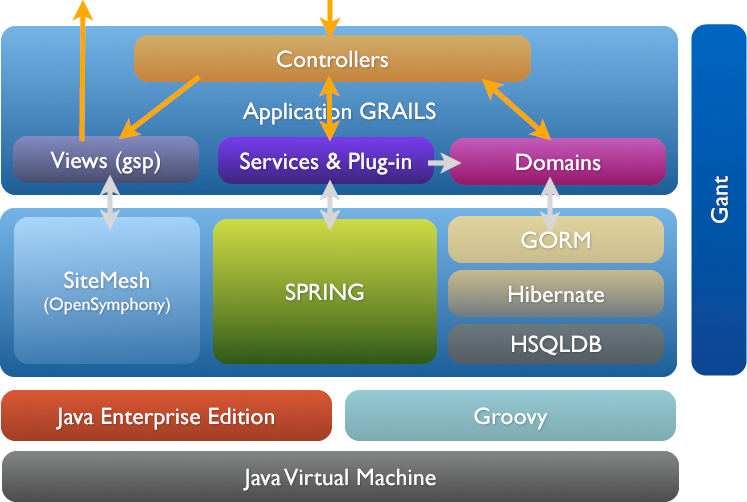
\includegraphics[width=100mm]{img/arch}
    \caption{Tecnolog\'ias que confirman la arquitectura de Grails}
    \label{arquitectura}

\end{figure}


\newpage
\section{Artefactos de Grails}
Grails consta de cuatro tipos de artefactos principales:
\begin{enumerate}
 \item Views
 \item Controllers
 \item Domains
 \item Services
\end{enumerate}

\subsection{Views}
Muestran informaci\'on al usuario de la aplicaci\'on. En Grails, las vistas existen en forma de archivos con extensi\'on \textit{gsp}. La informaci\'on es puesta en los \textit{gsp} a trav\'es de plantillas\footnote{Para los m\'as experimentados, llenar estas plantillas usan una sintaxis intermedia entre tags \textit{jstl} y tags de \textit{jsf}} y estas se llenan a trav\'es de controllers. 

\subsection{Controllers}
Se encargan de recibir peticiones desde las vistas, respondiendo con alguna de las siguientes formas:
\begin{enumerate}
 \item Renderizar una vista \textit{gsp},
 \item renderizar \textit{JSON},
 \item renderizar fragmentos \textit{HTML}
 \item etc.
\end{enumerate}

Asimismo los controllers deben lidiar con la l\'ogica de negocio de la aplicaci\'on, la cual puede colocarse dentro del mismo controller o en servicios inyectados\footnote{Checar Ap\'endice \ref{_depinject}}.

\subsection{Dominios}
Se encargan de describir el esquema de la base de datos a trav\'es de clases groovy. Grails se refiere al conjunto de estas clases y las funcionalidades agregadas por el framework\footnote{Cualquier funcionalidad relacionada con base de datos como CREATE, READ, UPDATE, DELETE y todas las que extienden de ellas} como \textit{GORM}.

\subsection{Servicios}
Se encargan de contener la l\'ogica de la aplicaci\'on y se conectan directamente con las clases de dominio.

Debido a la gran simplicidad de Grails, es com\'un que los desarrolladores escriban c\'odigo de acceso a base de datos y/o reglas de negocio dentro de los controladores. Y est\'a bien si as\'i les funciona, pero pierden las ventajas de algunas propiedades que los servicios tienen, por ejemplo:

\begin{itemize}
 \item Modularizaci\'on de c\'odigo
 \item Son transaccionales de forma predeterminada, es decir, si hay una operaci\'on a base de datos que necesite de varios pasos para completarse, y alguno de estos pasos falla, Grails ejecuta un rollback en la base de datos.
\end{itemize}



\begin{figure}[ht!]
    \begin{tikzpicture}[node distance = 2cm, auto]

        % Place nodes
        \node [block] (init) {controllers};
        \node [cloud, above of=init, node distance=2.5cm] (urls) {UrlMappings \newline(optional)};
        \node [cloud, left of=init, node distance=4.3cm] (views) {views};        
        \node [cloud, right of=init, node distance=4.1cm] (services) {services};    
        %\node [cloud, below of=views] (views2) {views};
        \node [cloud, below of=services] (domains) {domains};

        % Draw edges
        \path [line] (views) -- node [auto] {1.1 jquery, form} (urls);
        \path [line] (urls) -- node [auto] {1.2 (controlador y acci\'on decodificados)} (init);
    %     \path [line] (views) -- (views);
        \path [line] (init) -- node [auto] {2.1 invoke} (services);
        \path [line] (init) -- node [auto] {4 html,json,txt} (views);
        \path [line] (init) -- node [auto] {2.2 invoke} (domains);
        \path [line] (services) -- node [auto] {3 invoke} (domains);
        
    \end{tikzpicture}
    \caption{Artefactos de Grails funcionando}
\end{figure}